\documentclass[11pt]{article}

% ------
% LAYOUT
% ------
\textwidth 165mm %
\textheight 230mm %
\oddsidemargin 0mm %
\evensidemargin 0mm %
\topmargin -15mm %
\parindent= 10mm

\usepackage[dvips]{graphicx}
\usepackage{multirow,multicol}
\usepackage[table]{xcolor}

\usepackage{amssymb}
\usepackage{amsfonts}
\usepackage{amsthm}
\usepackage{amsmath}

\usepackage{subfigure}
\usepackage{minted}

\graphicspath{{./pix/}} % put all your figures here.

\begin{document}
\begin{center}
\Large{\textbf{ECE 595: Homework 1}}

Yi Qiao, Class ID

(Spring 2019)
\end{center}


\subsection*{Exercise 2}
\noindent\textbf{(a)} For a guassian distribution:

\begin{equation} \label{eq1}
\begin{split}
E[x] &=\int_{-\infty}^{\infty}x\frac{1}{\sqrt{2\pi\sigma^2}}e^{-\frac{(x-\mu)^2}{2\sigma^2}}dx \\
	&=\int_{-\infty}^{\infty}(x+\mu)\frac{1}{\sqrt{2\pi\sigma^2}}e^{-\frac{x^2}{2\sigma^2}}dx \\
	&=\int_{-\infty}^{\infty}x\frac{1}{\sqrt{2\pi\sigma^2}}e^{-\frac{x^2}{2\sigma^2}}dx+\int_{-\infty}^{\infty}\mu\frac{1}{\sqrt{2\pi\sigma^2}}e^{-\frac{x^2}{2\sigma^2}}dx \\
	&=0+\mu\frac{1}{\sqrt{2\pi\sigma^2}}\times\sigma\sqrt{2\pi} \\
	&=\mu
\end{split}
\end{equation}
\begin{equation} \label{eq2}
\begin{split}
Var[x] &=\int_{-\infty}^{\infty}(x-\mu)^2\frac{1}{\sqrt{2\pi\sigma^2}}e^{-\frac{(x-\mu)^2}{2\sigma^2}}dx \\
	&=\frac{1}{\sqrt{2\pi\sigma^2}}\int_{-\infty}^{\infty}x^2e^{-\frac{x^2}{2\sigma^2}}dx \\
	&let\ y = \frac{x}{\sigma},\ then\ dy=\frac{1}{\sigma}dx \\
	&=\frac{\sigma^3}{\sqrt{2\pi\sigma^2}}\int_{-\infty}^{\infty}y^2e^{-\frac{y^2}{2}}dy \\
	&=\sigma^2
\end{split}
\end{equation}

\noindent\textbf{(b)} Data generated and plotted as follows.
\begin{figure}[h]
\centering
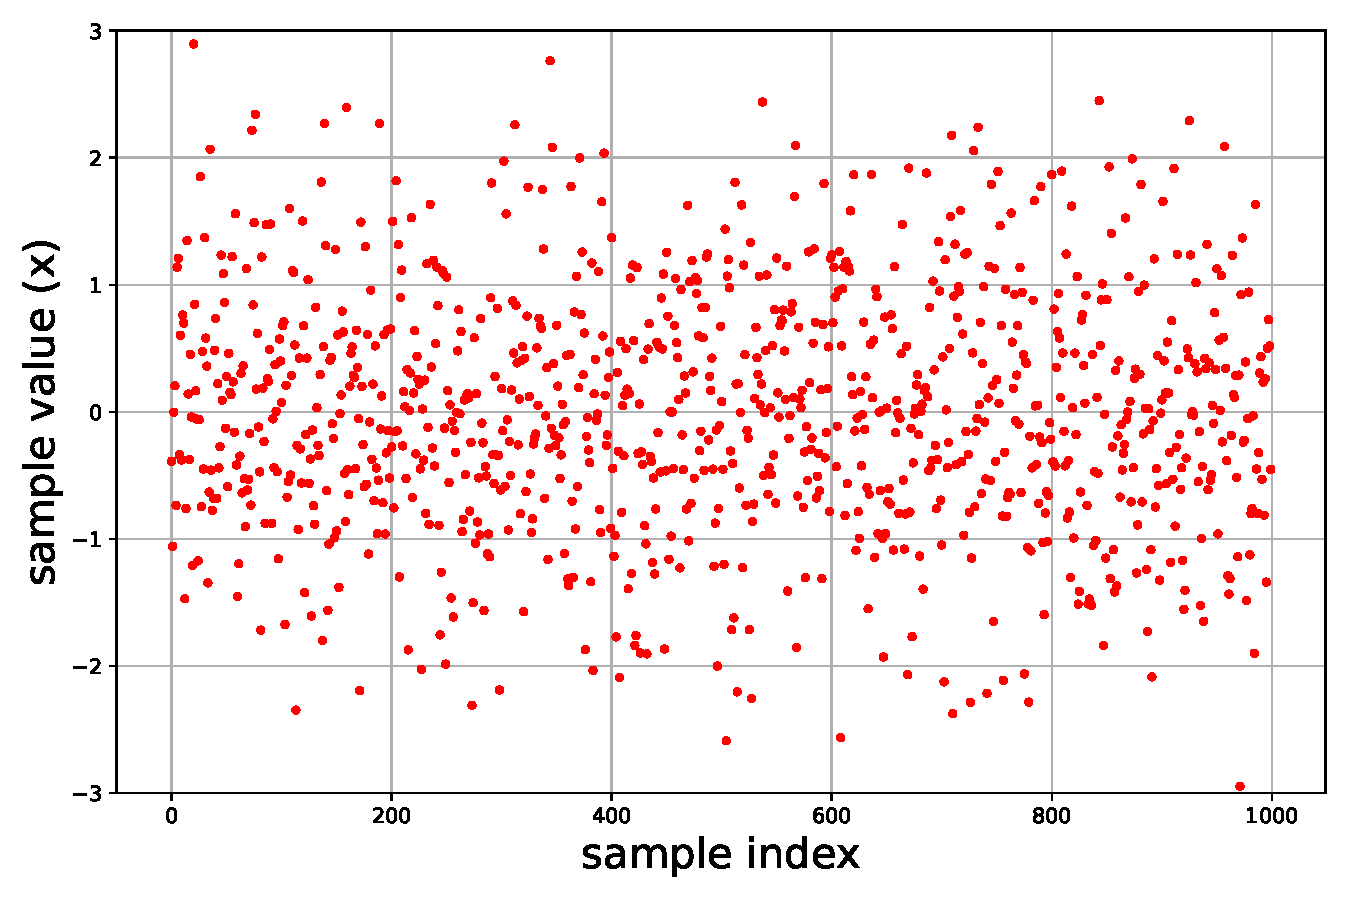
\includegraphics[width=0.5\linewidth]{exercise2_b}
\caption{Gussian random data.}
\label{fig: figure 1}
\end{figure}
\pagebreak

\noindent\textbf{(c)} \\

\textbf{(i)..(iv)} plots shown below

\begin{figure}[h]
\centering
\subfigure[4 bins]{
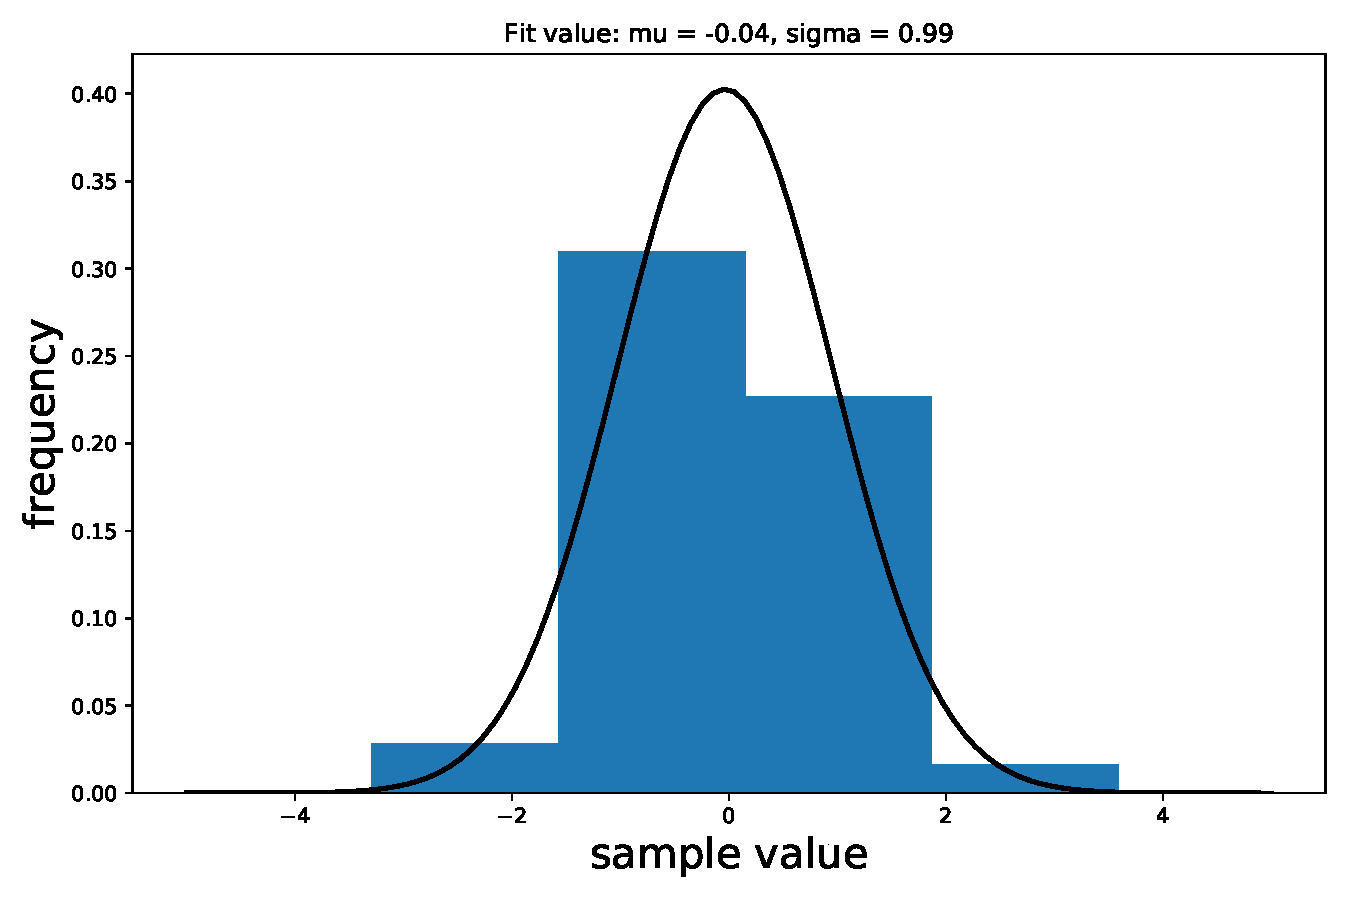
\includegraphics[width=0.47\linewidth]{exercise2_c1}
}
\subfigure[1000 bins]{
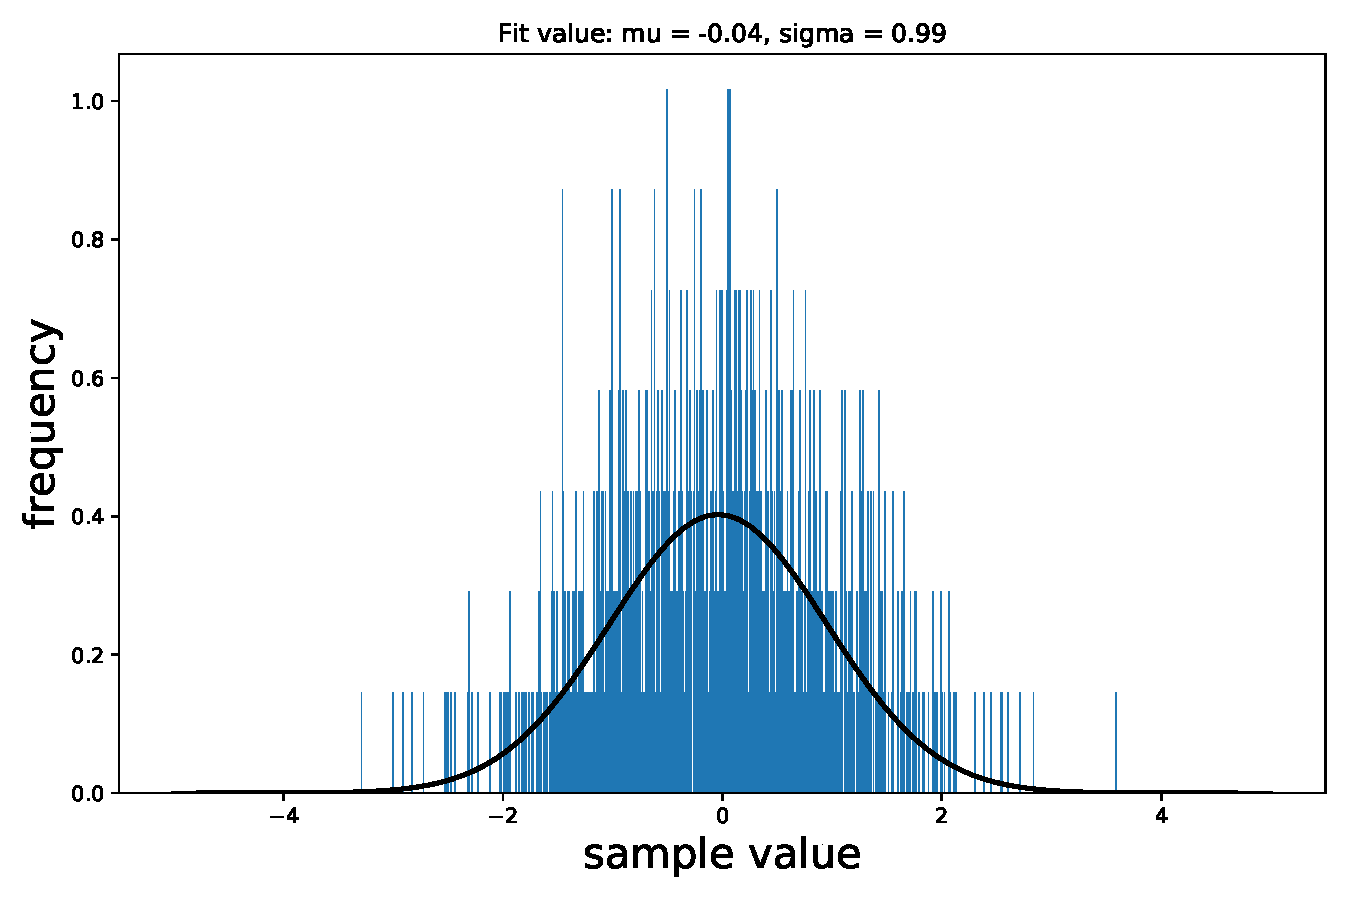
\includegraphics[width=0.47\linewidth]{exercise2_c2}
}
\end{figure}

\textbf{(v)}
TODO: fill this\\

\noindent\textbf{(d)}
compare to part (c), the histogram fits a lot better with the PDF
plots shown below

\begin{figure}[h]
\centering
\subfigure[Cross validation estimator of risk vs. \# of bins]{
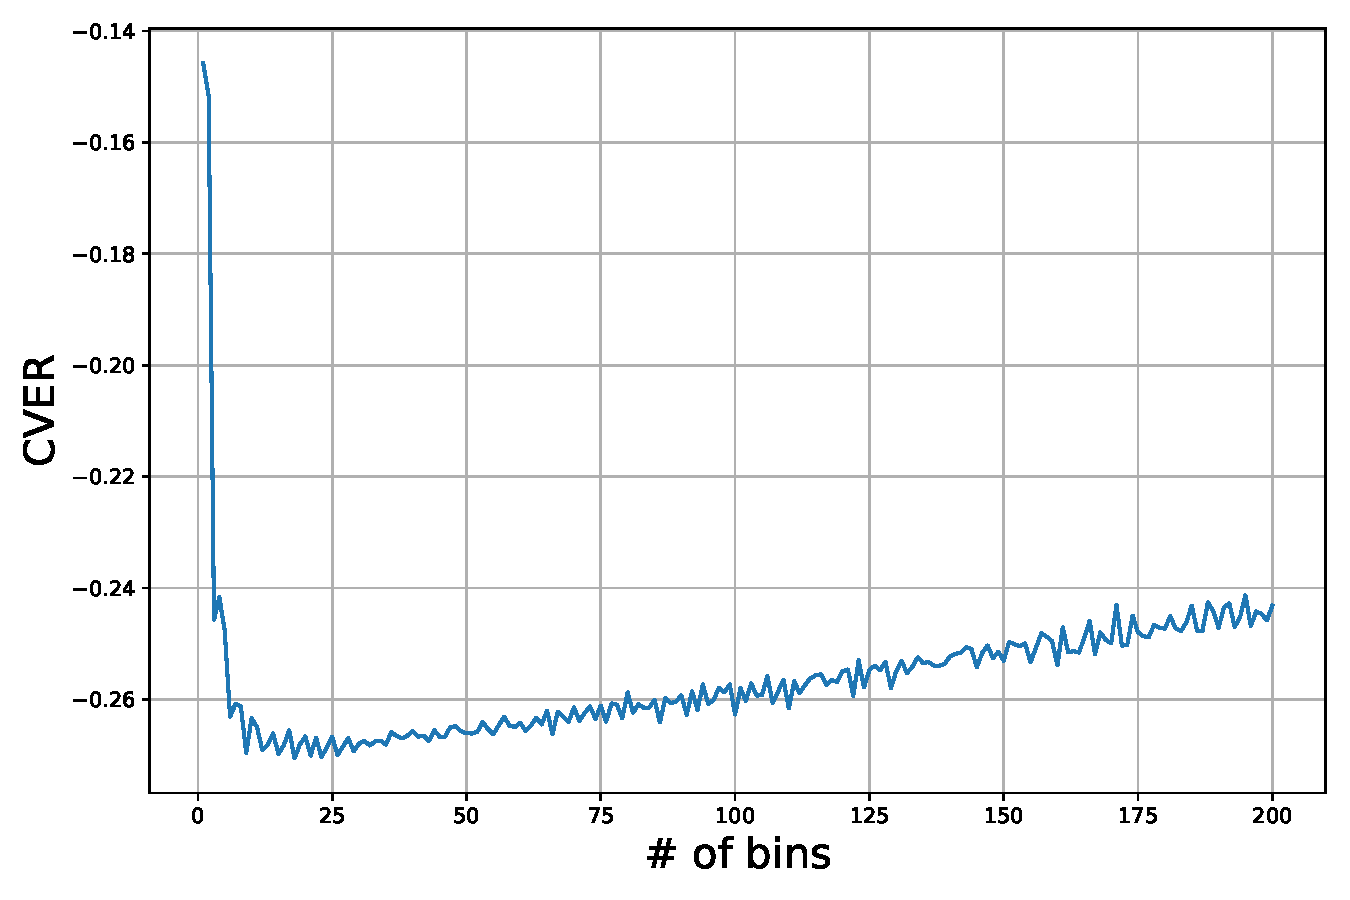
\includegraphics[width=0.47\linewidth]{exercise2_d1}
}
\subfigure[Histogram and PDF overlayed with optimized number of bins]{
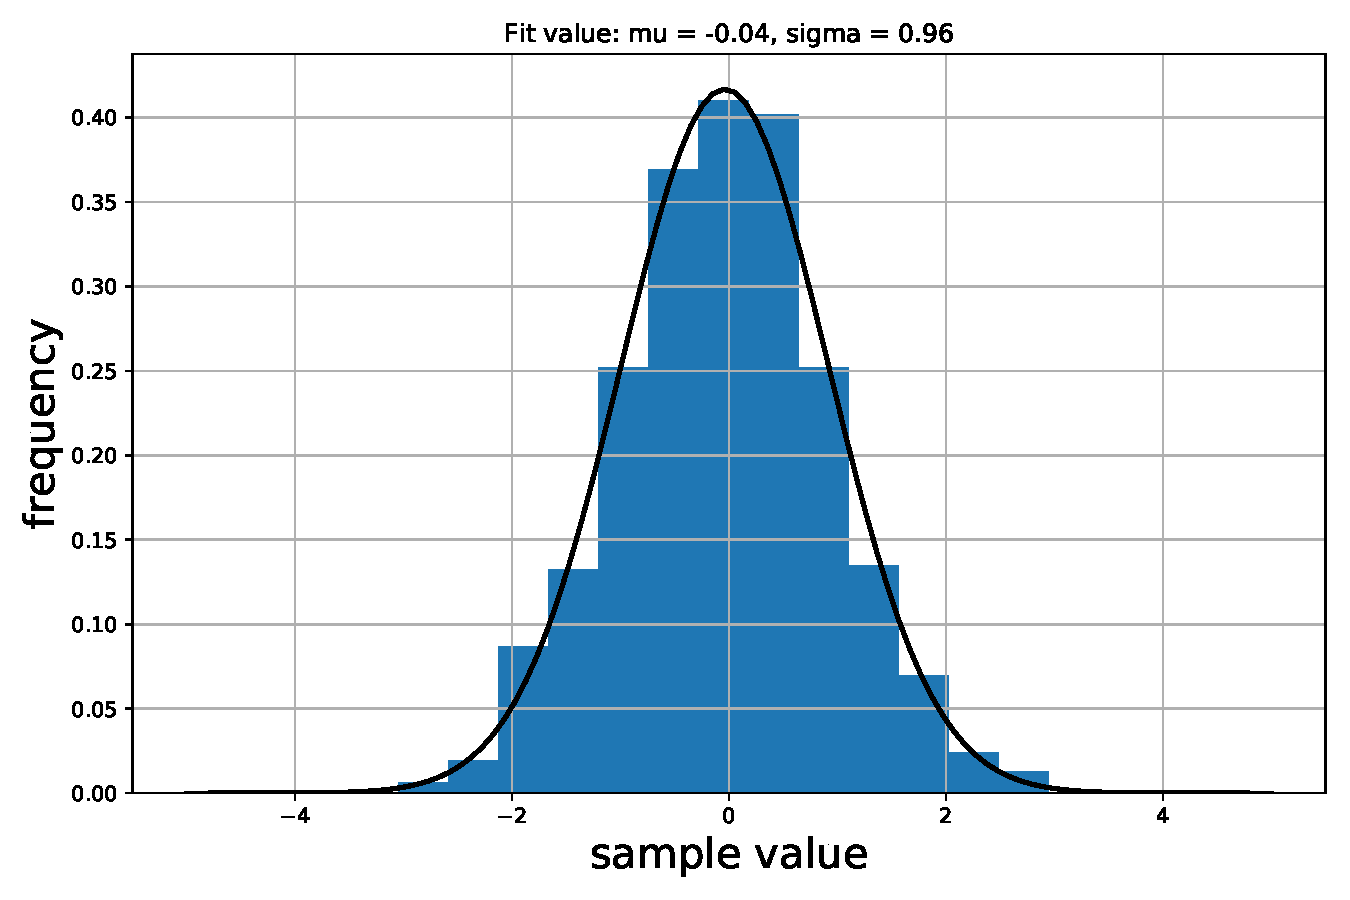
\includegraphics[width=0.47\linewidth]{exercise2_d2}
}
\end{figure}
\pagebreak

\subsection*{Exercise 3}

\noindent\textbf{(a)}
$$f_\textbf{X}(\textbf{x})=\frac{1}{\sqrt{2\pi^2|\pmb{\Sigma}|}}exp\{-\frac{1}{2}(\textbf{x}-\pmb{\mu})^T\pmb{\Sigma}^{-1}(\textbf{x}-\pmb{\mu})\}$$

\textbf{(i)}
plug in\\

\begin{center}
$\textbf{X}=\begin{bmatrix} X_1 \\ X_2 \end{bmatrix}$, 
$\textbf{x}=\begin{bmatrix} x_1 \\ x_2 \end{bmatrix}$,
$\pmb{\mu}=\begin{bmatrix} 2 \\ 6 \end{bmatrix}$,
  and  $\pmb{\Sigma}=\begin{bmatrix} 2 & 1 \\ 1 & 2 \end{bmatrix} $
\end{center}

we get\\
\begin{equation}
\begin{split}
f_{\begin{bmatrix} X_1 \\ X_2 \end{bmatrix}}\left(\begin{bmatrix} x_1 \\ x_2 \end{bmatrix}\right)&=\frac{1}{\sqrt{2\pi^2\begin{vmatrix} 2 & 1 \\ 1 & 2 \end{vmatrix}}}exp\left\{-\frac{1}{2}\begin{bmatrix} x_1-2 \\ x_2-6 \end{bmatrix}^T\begin{bmatrix} 2 & 1 \\ 1 & 2 \end{bmatrix}^{-1}\begin{bmatrix} x_1-2 \\ x_2-6 \end{bmatrix}\right\}\\
&=\frac{1}{\pi\sqrt{6}}exp\left\{-\frac{1}{3}\left((x_1-2)^2-(x_1-2)(x_2-6)+(x_2-6)^2\right)\right\}\\
\end{split}
\end{equation}

\textbf{(ii)}
plot shown below
\begin{figure}[h]
\centering
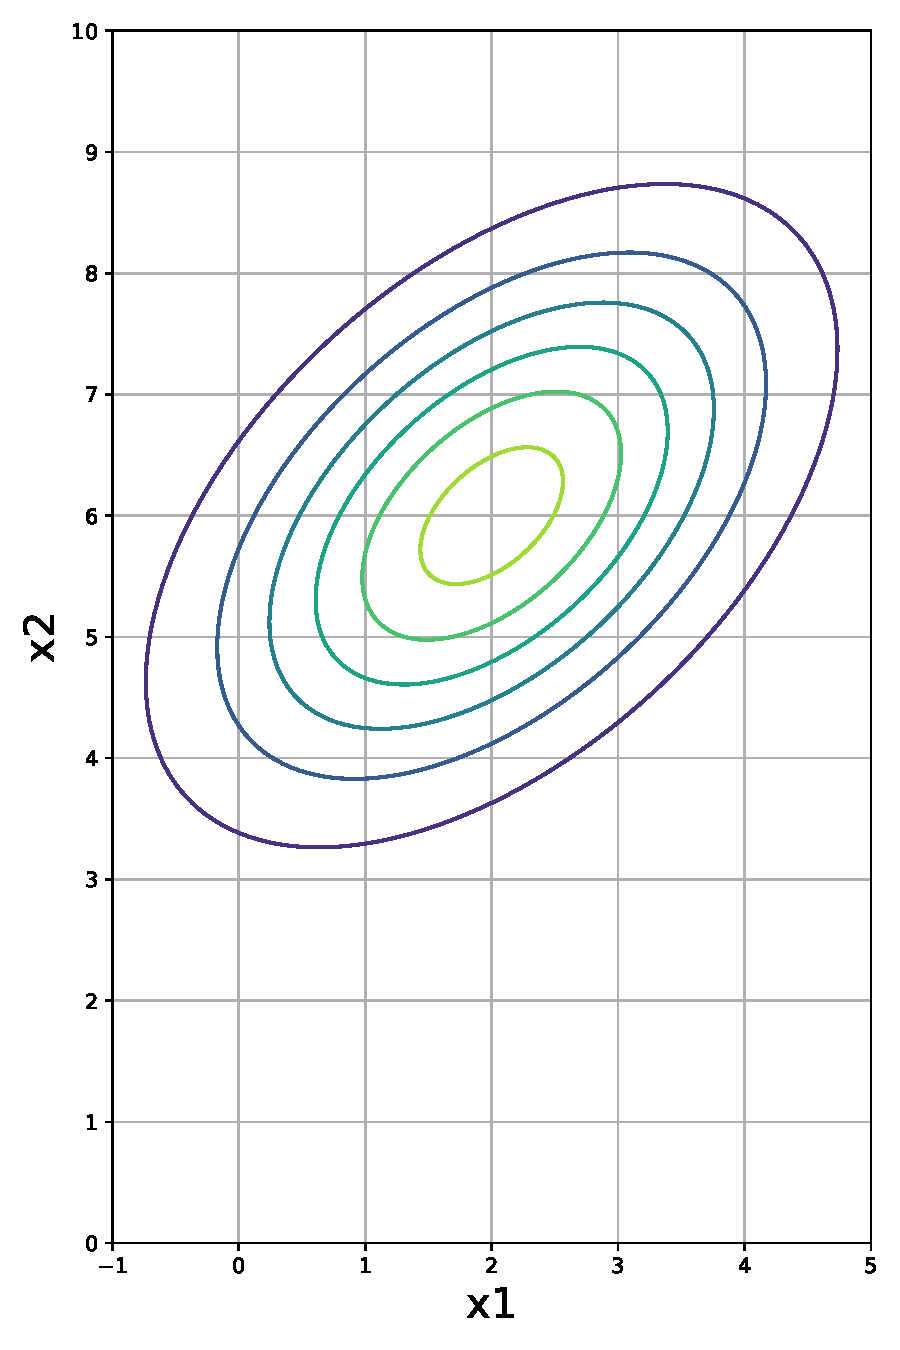
\includegraphics[width=0.45\linewidth]{exercise3_a}
\caption{Gussian random data}
\label{fig: figure 1}
\end{figure}
\pagebreak

\noindent\textbf{(b)}\\

\textbf{(i)}\\

To prove: $\pmb{\mu}_\textbf{Y}=b$
\begin{equation} \label{eq3}
\begin{split}
\pmb{\mu}_\textbf{Y}&=\mathbb{E}[\textbf{Y}]=\mathbb{E}[\textbf{A}\textbf{X}+\textbf{b}]=\mathbb{E}[\textbf{A}\textbf{X}]+\textbf{b} \\
&=\textbf{A}\mathbb{E}[\textbf{X}]+\textbf{b}\\
&since\ \textbf{X}\in \mathcal{N}(\textbf{0},\textbf{I}),\ \mathbb{E}[\textbf{X}]=\textbf{0}\\
&=\textbf{A}\textbf{0}+\textbf{b}\\
&=\textbf{b}
\end{split}
\end{equation}

To prove: $\pmb{\Sigma}_\textbf{Y}=\textbf{A}\textbf{A}^T$
\begin{equation} \label{eq4}
\begin{split}
\pmb{\Sigma}_\textbf{Y}&=\mathbb{E}[(\textbf{Y}-\pmb{\mu}_\textbf{Y})(\textbf{Y}-\pmb{\mu}_\textbf{Y})^T]\\
&=\mathbb{E}[\textbf{AX}\textbf{X}^T\textbf{A}^T]\\
&=\textbf{A}\mathbb{E}[\textbf{XX}^T]\textbf{A}^T\\
&=\textbf{A}(\textbf{I}+\textbf{0})\textbf{A}^T\\
&=\textbf{AA}^T
\end{split}
\end{equation}

\textbf{(ii)}
To prove: $\pmb{\Sigma}_\textbf{Y}$ is symmetric and positive semi-definite\\
\begin{equation} \label{eq5}
\begin{split}
\pmb{\Sigma}_{\textbf{Y}ij}&=\Sigma_{x=1}^n\textbf{A}_{ix}\textbf{A}^T_{xj}\\
&=\Sigma_{x=1}^n\textbf{A}_{jx}\textbf{A}_{xi}^T\\
&=\pmb{\Sigma}_{\textbf{Y}ji}\\
&thus\ symmetric \\
\textbf{x}^T\pmb{\Sigma}_\textbf{Y}\textbf{x}&=\textbf{x}^T\textbf{AA}^T\textbf{x}\\
let\ \textbf{y}=\textbf{x}^T\textbf{A}\\
&=\textbf{yy}^T\\
&=\|\textbf{y}\|^2 \ge 0\\
&thus\ positive\ semi-definite
\end{split}
\end{equation}

\textbf{(iii)}
$$Null(\textbf{A}) = \textbf{0}$$

\textbf{(iv)}
By inspection,
$$b=\pmb{\mu}_\textbf{Y}=\begin{bmatrix}2\\6\end{bmatrix}$$

By Cholesky decomposition,
$$\pmb{\Sigma}_\textbf{Y}=\textbf{A}\textbf{A}^T$$
$$\textbf{A}=\begin{bmatrix}
\sqrt{2}	&0\\
\frac{\sqrt{2}}{2}	&\frac{\sqrt{6}}{2}
\end{bmatrix}$$
\pagebreak

\noindent\textbf{(c)}\\

\textbf{(i)} Data points drawn from 2D standard guassian distribution are shown below.
\begin{figure}[h]
\centering
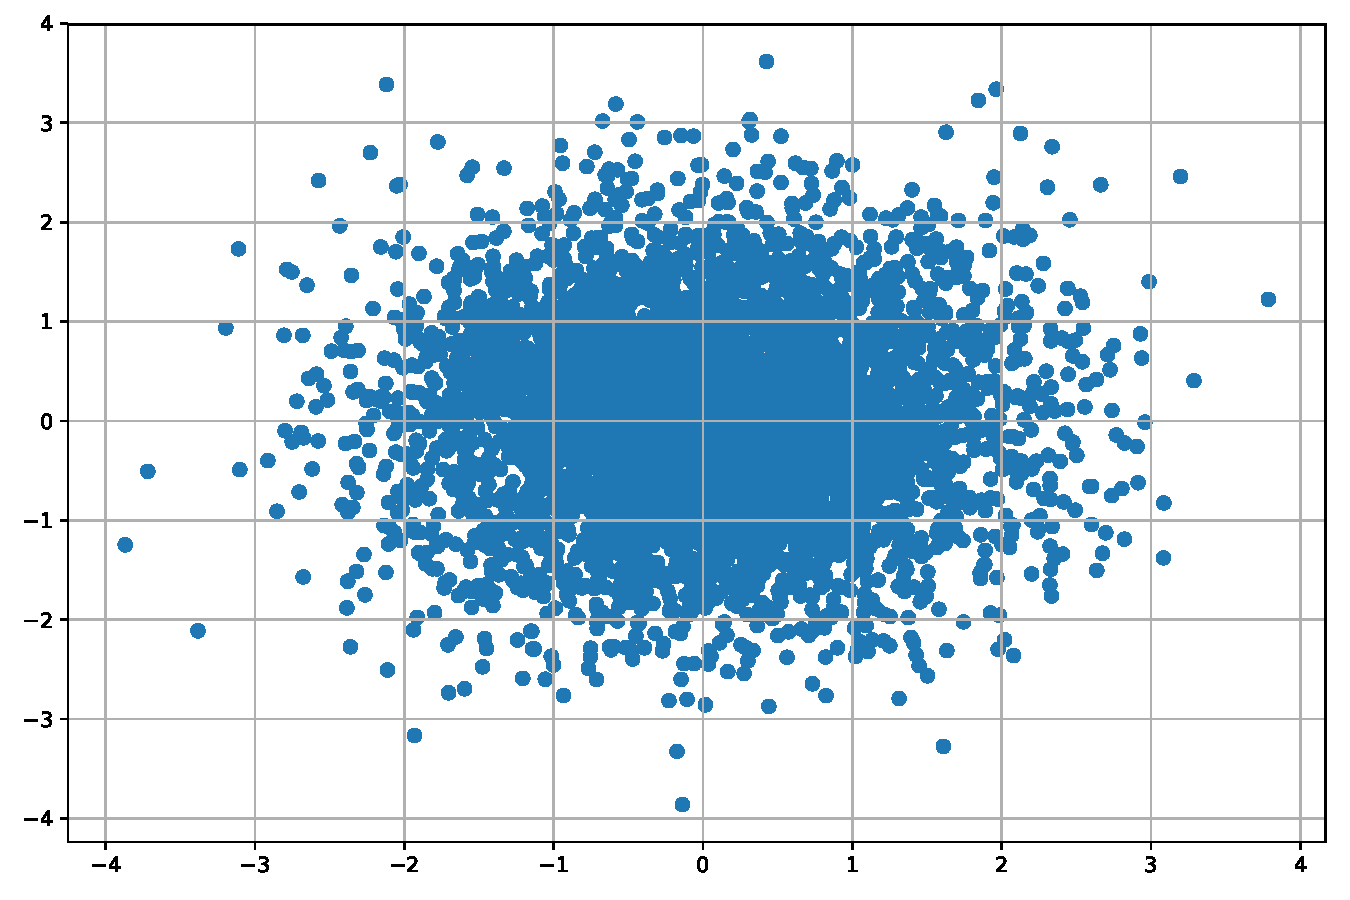
\includegraphics[width=0.45\linewidth]{exercise3_c1}
\caption{2D standard Gussian random data}
\label{fig: figure 3.2}
\end{figure}

\textbf{(ii)} After applying the affine transformation, the data plot shown below.
\begin{figure}[h]
\centering
\subfigure[After applying affine transformation]{
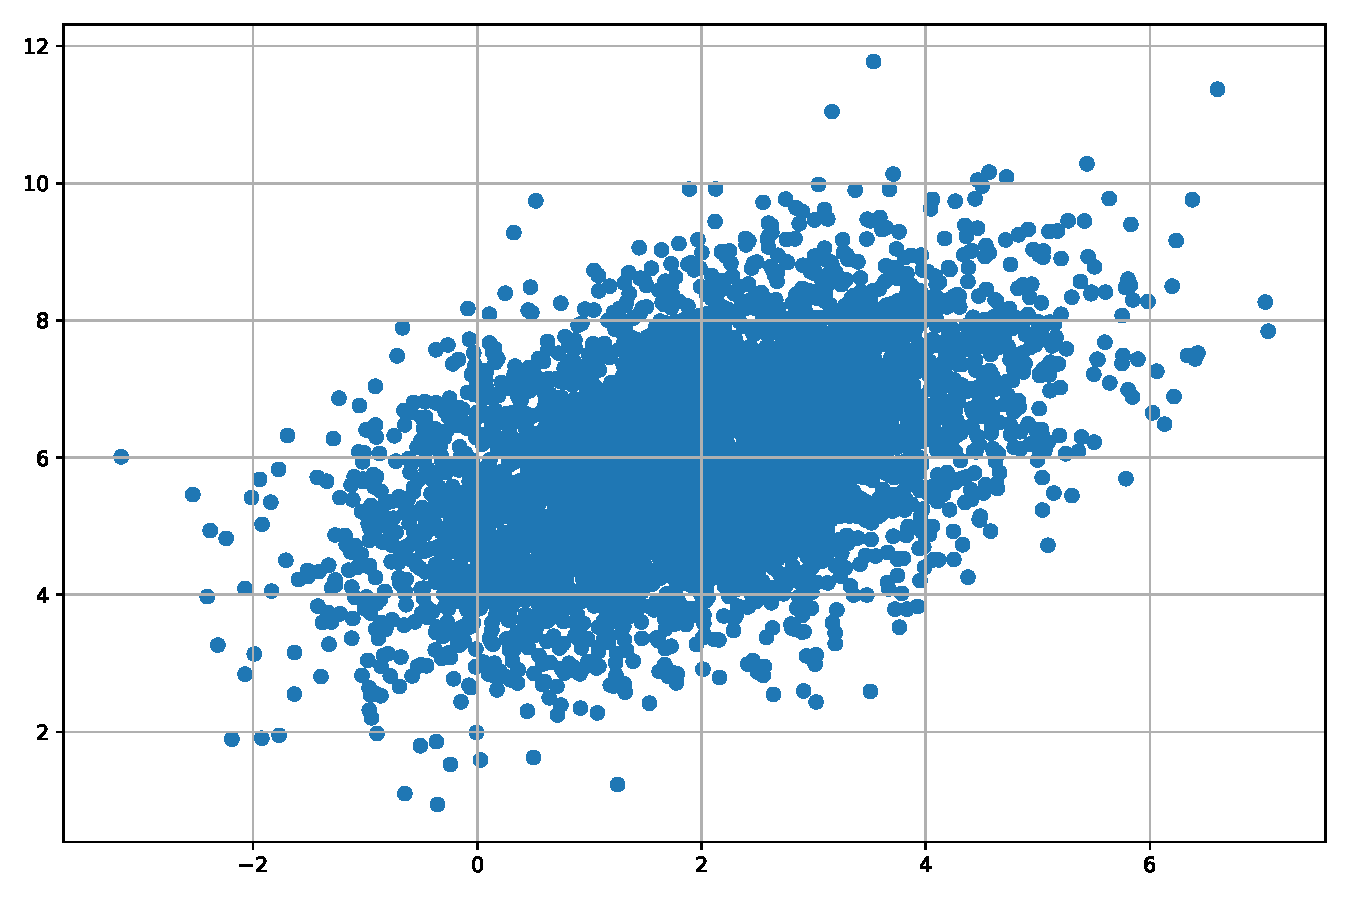
\includegraphics[width=0.45\linewidth]{exercise3_c2}
}
\subfigure[After applying transform get from eigen]{
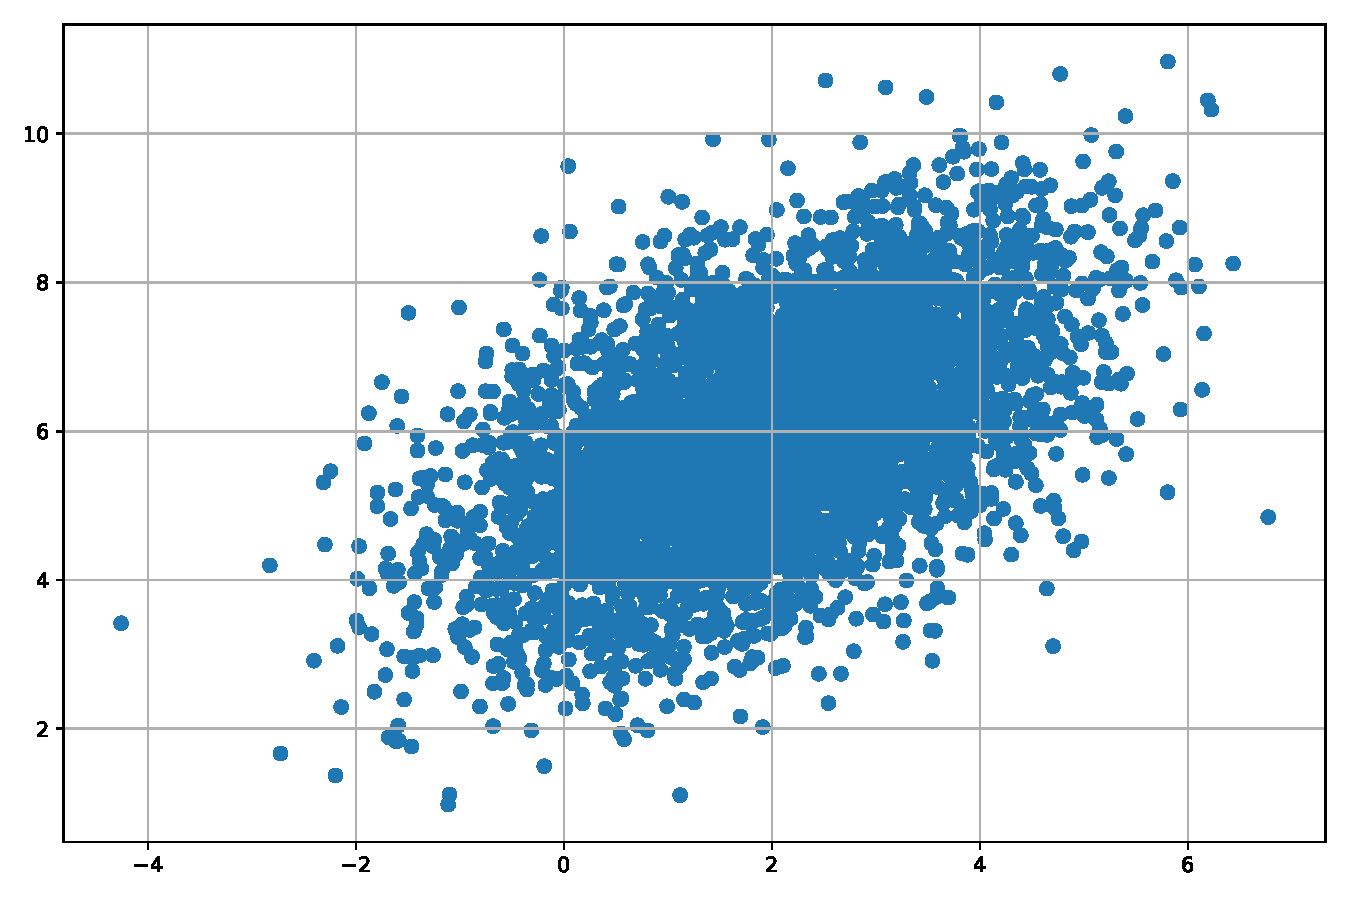
\includegraphics[width=0.45\linewidth]{exercise3_c3}
}
\label{fig: figure 3.3}
\end{figure}

\begin{figure}[h]
\centering
\subfigure[Cross validation estimator of risk vs. \# of bins]{
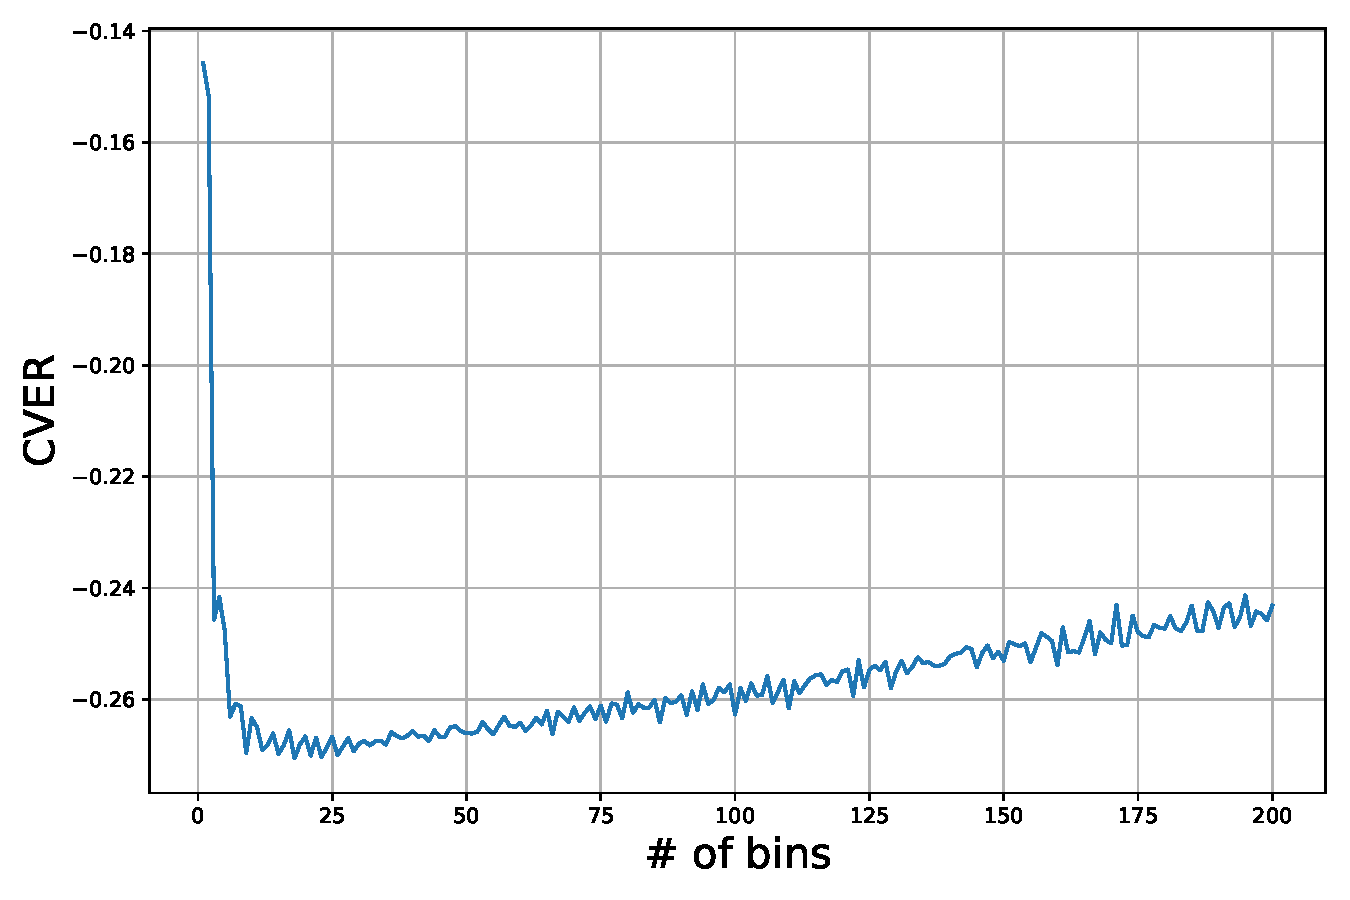
\includegraphics[width=0.47\linewidth]{exercise2_d1}
}
\subfigure[Histogram and PDF overlayed with optimized number of bins]{
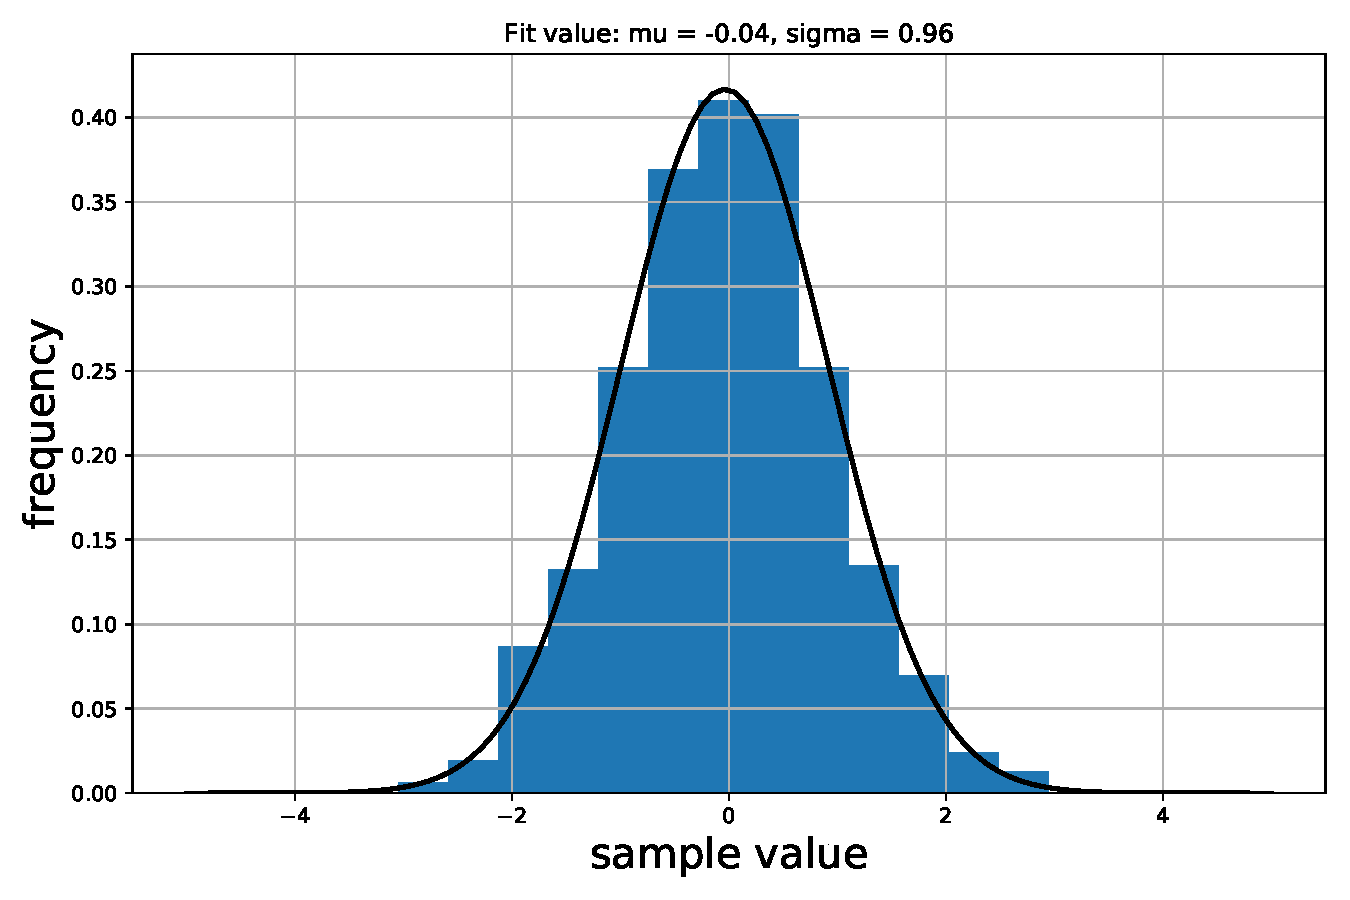
\includegraphics[width=0.47\linewidth]{exercise2_d2}
}
\end{figure}
\textbf{(iii)} From my favorite python and numpy, for the data above:
$$\pmb{\mu}_\textbf{Y}=\begin{bmatrix}
2.003\\
6.004
\end{bmatrix}$$
$$\pmb{\Sigma}_\textbf{Y}=\begin{bmatrix}
2.017& 1.050\\
1.050& 2.074
\end{bmatrix}$$
\pagebreak
\subsection*{Exercise 4}
\noindent\textbf{(a)}\\
\textbf{Proof}
\begin{equation} \label{4.a}
\begin{split}
\left|\textbf{x}^T\textbf{Ay}\right|&=\left|\sum_{i}\sum_{j}a_{ij}x_iy_j\right|\\
&\le\sum_i\sum_j\left|a_{ij}\right|\left|x_i\right|\left|y_j\right|\\
&=\sum_i\sum_j(\left|a_{ij}\right|^\frac{1}{2})^2\left|x_i\right|\left|y_j\right|\\
&by\ Cauchy\ Schwarz\\
&\le\sqrt{\sum_i\sum_j\left|a_{ij}\right|\left|x_i\right|^2}\sqrt{\sum_i\sum_j\left|a_{ij}\right|\left|y_j\right|^2}\\
&=\sqrt{\sum_i\left|x_i\right|^2\sum_j\left|a_{ij}\right|}\sqrt{\sum_j\left|y_j\right|^2\sum_i\left|a_{ij}\right|}\\
&\le\sqrt{\sum_i\left|x_i\right|^2C}\sqrt{\sum_j\left|y_j\right|^2R}\\
&=\sqrt{RC}||x||_2||y||_2\\
\end{split}
\end{equation}

\noindent\textbf{(b)}\\

\textbf{(i)}
For a invertible $n\times n$ matrix \textbf{A}\\
\begin{equation} \label{eq6}
\begin{split}
\textbf{A}&=\textbf{PDP}\\
\textbf{A}^{-1}&=(\textbf{PDP}^{-1})^{-1}\\
&=\textbf{P}^{-1}\textbf{D}^{-1}\textbf{P}\\
\end{split}
\end{equation}

Since A is positive definite, $\lambda_i > 0\ for\ 1\le i\le n$, $\textbf{D}$ is invertible.\\

Thus \textbf{A} is also invertible.\\

\textbf{(ii)}
$$f\left(\begin{bmatrix}
x1\\x2
\end{bmatrix}\right) = x_1^2-x_2^2$$

the Hessian of this function is\\

$$\begin{bmatrix}
2&0\\0&-2
\end{bmatrix}
$$

which is invertible but not positive definite\\

\pagebreak
\textbf{(iii)}
If a matrix is invertible while positive semi-definite, the matrix is positive definite.

By definition of positive semi-definite, $\textbf{xAx}^T\ge 0$, and for a eigenvalue of $\textbf{A}$, $\lambda_i$, $\lambda_i\textbf{u}_i=\textbf{Au}_i$ 

So, 
\begin{equation} \label{eq7}
\begin{split}
\textbf{u}_i^T\textbf{A}\textbf{u}_i&=\lambda_i\\
\lambda_i&\ge 0\\
\end{split}
\end{equation}

If the matrix is invertible, it cannot have $\lambda_i = 0$.

So, $\lambda_i>0$, thus $\textbf{xAx}^T>0$.

The matrix \textbf{A} is positive definite.\\

\noindent\textbf{(c)}
To prove: $(\exists \textbf{A}^\dagger)\ \textbf{AA}^\dagger \textbf{A} = \textbf{A}$

\begin{equation} \label{eq8}
\begin{split}
\textbf{A}&=\textbf{U}\pmb{\Lambda}\textbf{U}^T\\
\textbf{AA}^\dagger \textbf{A}&=\textbf{U}\pmb{\Lambda}\textbf{U}^T\textbf{A}^\dagger\textbf{U}\pmb{\Lambda}\textbf{U}^T\\
&=\textbf{U}\pmb{\Lambda}\textbf{U}^T\\
&simplify\\
\textbf{U}^T\textbf{A}^\dagger\textbf{U}\pmb{\Lambda}&=\pmb{\Lambda}\pmb{\Lambda}^-\\
\textbf{A}^\dagger&=\textbf{U}\pmb{\Lambda}^{-}\textbf{U}^T\\
\end{split}
\end{equation}

Since \textbf{A} is symmetric, it is guaranteed that can be decompose,
thus $\textbf{A}^\dagger$ exist.

\pagebreak
\section*{Code}
\subsection*{Exercise2}
\inputminted{python}{py/exercise2.py}
\pagebreak

\subsection*{Exercise3 (a)}
\inputminted{python}{py/exercise3_a.py}
\pagebreak

\subsection*{Exercise3 (c)}
\inputminted{python}{py/exercise3_a.py}
\end{document}

